\documentclass[12]{article}
\usepackage{hyperref}
\usepackage{graphicx}
\usepackage{listings}
\usepackage{color}

\definecolor{dkgreen}{rgb}{0,0.6,0}
\definecolor{gray}{rgb}{0.5,0.5,0.5}
\definecolor{mauve}{rgb}{0.58,0,0.82}

\lstset{frame=tb,
  language=C++,
  aboveskip=3mm,
  belowskip=3mm,
  showstringspaces=false,
  columns=flexible,
  basicstyle={\small\ttfamily},
  numbers=none,
  numberstyle=\tiny\color{gray},
  keywordstyle=\color{blue},
  commentstyle=\color{dkgreen},
  stringstyle=\color{mauve},
  breaklines=true,
  breakatwhitespace=true,
  tabsize=3
}

\title{ACSL TurtleBot3 e-Manual}

\date{June 2020}
\renewcommand\thesection{\arabic{section}}
\renewcommand\thesubsection{\thesection.\arabic{subsection}}

\begin{document}

\makeatletter
    \begin{titlepage}
        \begin{center}
            
\includegraphics[width=0.7\linewidth]{images/ACSL_Logo.jpg}\\[4ex]
            {\huge \bfseries  \@title }\\[52ex]  
            {\large \@date}
        \end{center}
    \end{titlepage}
\makeatother

\tableofcontents
\newpage

\section*{Abstract}
   
This guide documents the changes made to TurtleBot3 software to meet the requirements of ACSL research group. It contains instructions on setting up the robot and code documentation.
       
\addcontentsline{toc}{section}{Abstract}
\newpage

\section{Overview and Setup}

TurtleBot3 is a small ROS-based mobile robot. The TurtleBot3 can be customized by changing the source code and addition of new hardware. TurtleBot3 Waffle Pi is equipped with a Raspberry Pi Camera Module (v2), a 360-degree Laser Distance Sensor (LDS) and Dynamixel XM430 210-T motors.

TurtleBot3 architecture is described in the following image.\\

\begin{center}
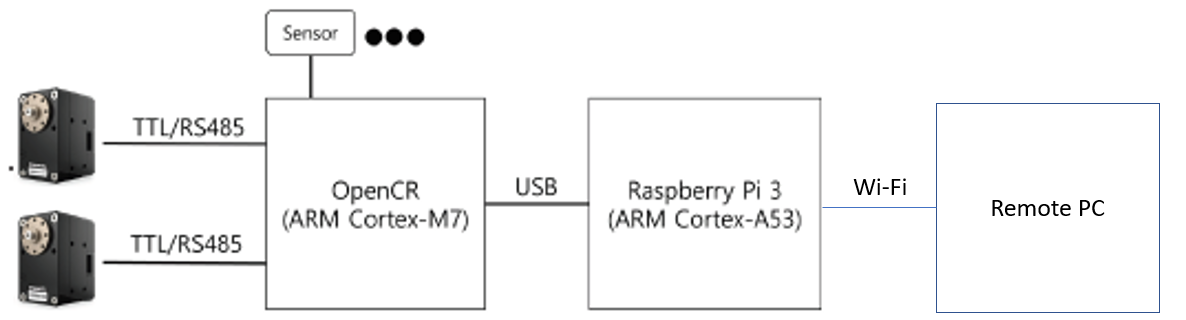
\includegraphics[width=0.7\linewidth]{images/tb3_architecture.png}\\
\end{center}

The four major components of TurtleBot3 are 
\begin{enumerate}
	\item {Raspberry Pi 3B+ Single Board Computer (SBC).}
	\item {OpenCR Embedded System Board.}
	\item {LDS and Camera Sensors.}
	\item {Dynamixel Actuators.}
\end{enumerate}

Raspberry Pi has a WiFi module built onto the board which connects to a computer, known as the Remote PC. Remote PC is used to send commands for SLAM and Navigation to TB3 and visualization of the sensor data is also performed on the remote PC.

There is a one time setup that needs to be performed on the Remote PC, Raspberry Pi and OpenCR board. Most of the software is located in the form of a binary file that is burnt to the EEPROM of the STM32F746 chip on the OpenCR board. As the software used for ACSL projects is custom, it is burnt using Arduino IDE.
 
\subsection{Remote PC Setup}

To begin you will need to install the appropriate ROS version on your remote PC. The remote PC will be running ROS Melodic which is backwards compatible with ROS Kinetic (The Distribution we will flash on the Turtlebot's on board computer).

The following page from the ROBOTIS E manual describes the process for adding and installing all necessary packages to your ROS Environment.

\url {https://emanual.robotis.com/docs/en/platform/turtlebot3/pc_setup/#network-configuration} \\\\

The next step is to configure network settings for permanent use. The Remote PC will be controlling the turtlebot pc via wifi using SSH protocol. Steps for configuring the wifi on the remote pc can be found here.

\url {https://emanual.robotis.com/docs/en/platform/turtlebot3/pc_setup/#install-ros-1-on-remote-pc} \\

For this project we will use the Linksys Router on the \textbf{Linksys04294} network. It is helpful to write down the IP address of the remote pc, since you will need it later to setup the turtlebot pc network settings.\\\\

\subsection{Rasberry Pi SBC Setup}

Now it is time to look at the turtlebot SBC. For the turtlebot 3 Waffle Pi model, the on board PC is a raspberry PI. This step requires a micro SD card with adapter, a monitor with an HDMI input, a USB keyboard and mouse, and a power source for the turtlebot. ROBOTIS provides a prebuilt desktop environment for the turtlebot with ROS kinetic. Instructions for flashing this distribution can be found here (\textbf{Step 6.2.1.2 Install Linux Based on Raspbian, Do not use the other two methods.}).\\

\url {https://emanual.robotis.com/docs/en/platform/turtlebot3/raspberry_pi_3_setup/#raspberry-pi-3-setup}

\subsection{OpenCR Setup}

The original source code for TurtleBot3 used the inbuilt PID controller of the Dynamixel XM430 210-T actuators. However, to benchmark the performance of the controllers, the control is shifted from the motors to higher level software such as Simulink or a custom ROS node.

The source code for OpenCR can be downloaded by cloning the following repository.

\url {https://github.com/hanyiabc/ASCL_turtlebot3.git}

Arduino IDE can be used to burn the turtlebot3\_core.ino file located in ACSL\_turtlebot3/src/turtlebot3\_core directory. Instructions for setting up the Arduino IDE for TurtleBot3 can be found in the following link.

\url {https://emanual.robotis.com/docs/en/parts/controller/opencr10/#arduino-ide}

\newpage

\section{Torque Control using Dynamixel}
       
Dynamixel is a microcontroller based actuator with in-built PID controller. OpenCR communicates with Dynamixel using packet communication via TTL/RS45 ports. 

Hardware level abstraction is achieved via Dynamixel SDK library available in several programming languages. (CPP used in our case.)
Dynamixel register addresses and byte sizes for both RAM and EEPROM memory provided in control table. RAM is most frequently used memory for robot applications, while startup settings are stored on EEPROM.

The Control Table is a structure that consists of multiple Data fields to store status or to control the device. Users can check current status of the device by reading a specific Data from the Control Table with Read Instruction Packets. WRITE Instruction Packets enable users to control the device by changing specific Data in the Control Table. Packet sizes range from 1 – 4 bytes.

Following is a snapshot of the Dynamixel EEPROM Control Table. Each data in the Control Table is restored to initial values when the device is turned on. Default values in the EEPROM area (addresses 0-63) are initial values of the device (factory default settings). If any values in the EEPROM area are modified by a user, modified values will be restored as initial values when the device is turned on. Initial Values in the RAM area are restored when the device is turned on.

\begin{center}
	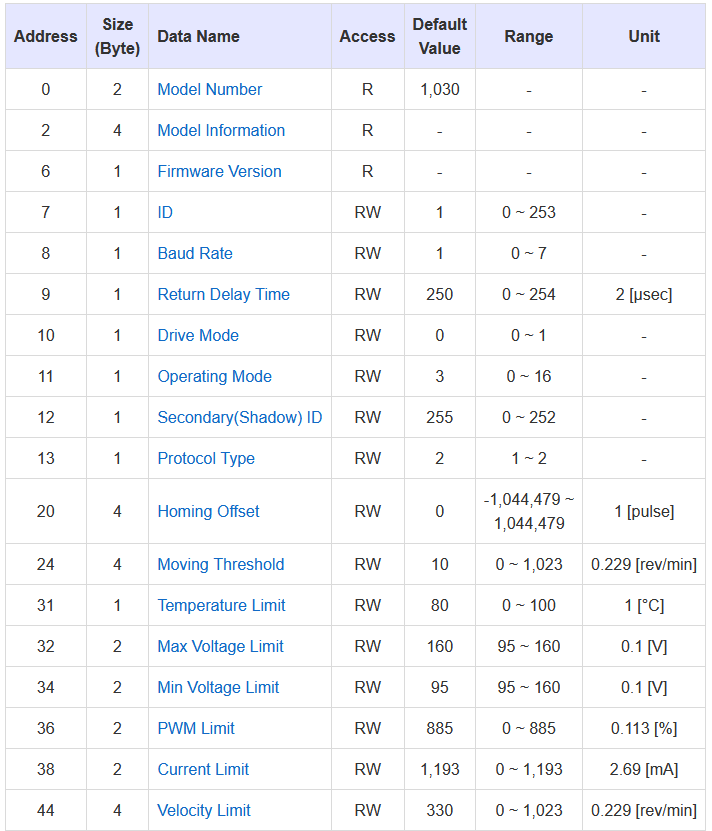
\includegraphics[width=0.7\linewidth]{images/dxl_eeprom.png}\\
\end{center}

For the purpose of torque control, the operating mode of the dynamixel motor needs to be set to \textbf{MODE 0}. This can be done using the motor setup code in the git repository.

Once the operating mode is set. The OpenCR code is change to write torque values to the Dynamixel RAM addresses, when the robot is live. The addresses that are useful for this purpose are given in the image below.

\begin{center}
	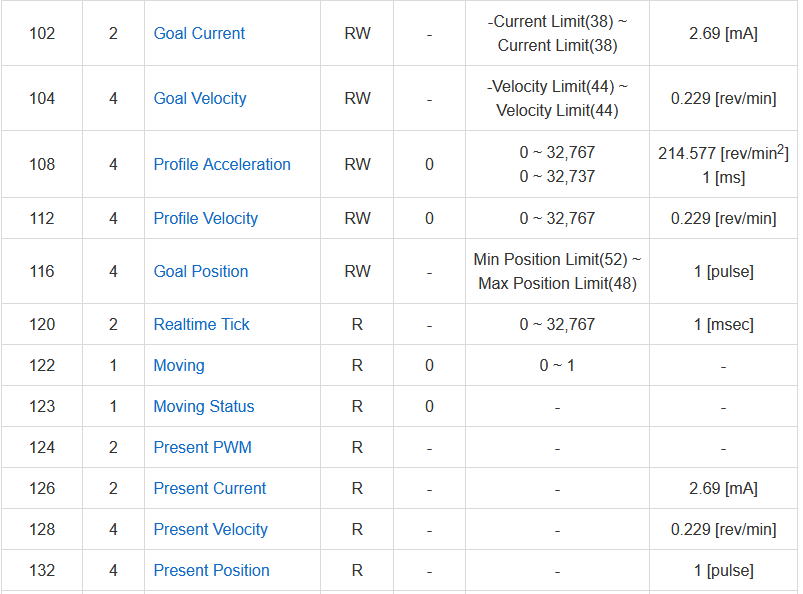
\includegraphics[width=\linewidth]{images/dxl_control_table.png}\\
\end{center}

The following method is added to the TurtleBot3MotorDriver class, which takes in input torque value and converts it into appropriate register values for writing to the appropriate addresses.

\begin{lstlisting}
bool TurtleBot3MotorTorqueDriver::controlMotor(float *torque)
{
        bool dxl_comm_result = false;

        uint16_t wheel_current_cmd[2];
        wheel_current_cmd[LEFT] = CURRENT_TO_OUTPUT(TORQUE_TO_CURRENT(torque[LEFT]));
        wheel_current_cmd[RIGHT] = CURRENT_TO_OUTPUT(TORQUE_TO_CURRENT(torque[RIGHT]));

        wheel_current_cmd[LEFT] = constrain(wheel_current_cmd[LEFT], -dynamixel_limit_max_current_, dynamixel_limit_max_current_);
        wheel_current_cmd[RIGHT] = constrain(wheel_current_cmd[RIGHT], -dynamixel_limit_max_current_, dynamixel_limit_max_current_);

        dxl_comm_result = writeTorque((int16_t)wheel_current_cmd[LEFT], (int16_t)wheel_current_cmd[RIGHT]);
        if (dxl_comm_result == false)
            return false;

        return true;
}
\end{lstlisting}

This conversion is based on a linear approximation of the actuator performance graph.

\begin{center}
	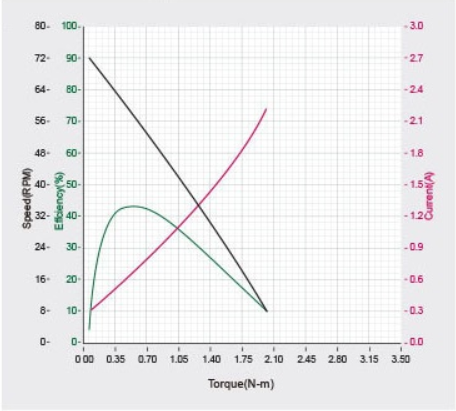
\includegraphics[width=\linewidth]{images/xm430_performance.png}\\
\end{center}

\begin{lstlisting}
bool TurtleBot3MotorTorqueDriver::writeTorque(int16_t left_value, int16_t right_value)
{
    bool dxl_addparam_result;
    int8_t dxl_comm_result;

    dxl_addparam_result = groupSyncWriteTorque_->addParam(left_wheel_id_, (uint8_t *)&left_value);
    if (dxl_addparam_result != true)
        return false;

    dxl_addparam_result = groupSyncWriteTorque_->addParam(right_wheel_id_, (uint8_t *)&right_value);
    if (dxl_addparam_result != true)
        return false;

    dxl_comm_result = groupSyncWriteTorque_->txPacket();
    if (dxl_comm_result != COMM_SUCCESS)
    {
        Serial.println(packetHandler_->getTxRxResult(dxl_comm_result));
        return false;
    }

    groupSyncWriteTorque_->clearParam();
    return true;
}
\end{lstlisting}

\newpage

\section{Custom controller in Simulink}

\end{document}
